\subsection{Membership Determination}

In order to properly characterize a SC, it's member stars must be properly identified to avoid including field stars not bound to the cluster in question for the ensuing CMD analysis. As a result, cluster membership determination algorithms have received a large amount of attention in recent years. For this project we implement a membership determination pipeline using HDBSCAN, an improvement over the DBSCAN clustering algorithm by assembling minimum spanning trees and subsequently compacting them into a set of "groupings," from which stellar clusters are identified. HDBSCAN has been used in recent works with a high rate of success in both identifying previously unknown SCs as well as expanding on known clusters' membership lists \autocite{huntImprovingOpenCluster2021,sanchez-sanjuanKinematicStudyOrion2024a,tarricqStructuralParameters3892022a}. 

\subsubsection{Gaia DR3 Data Selection}

Our HDBSCAN pipeline operates on the Gaia DR3 (GDR3) \autocite{gaiacollaborationGaiaDataRelease2023a} 5D astrometric phase space ($\alpha, \delta, \omega, \mu_{\alpha} \cos{\delta}, \mu_{\delta}$); radial velocities are not included in order to maximize our sample size, as few stars within the GDR3 catalog include radial velocity measurements. For each of the four clusters analyzed for this work we selected all stars within a conical field centered on the cluster reported center. The search radius was taken as a multiple of the literature reported cluster radius: $\texttt{max}\left(10 \cdot R_{50, \ \mathrm{UCC}}, \ 2 \cdot R_{\mathrm{tot}, \ \mathrm{HR24}}\right)$, where $R_{50, \ \mathrm{UCC}}$ is the half-member radius reported in the UCC, and $R_{\mathrm{tot}, \ \mathrm{HR24}}$ is the tidal radius reported by \cite{huntImprovingOpenCluster2024a}.

\begin{figure}[!ht]
    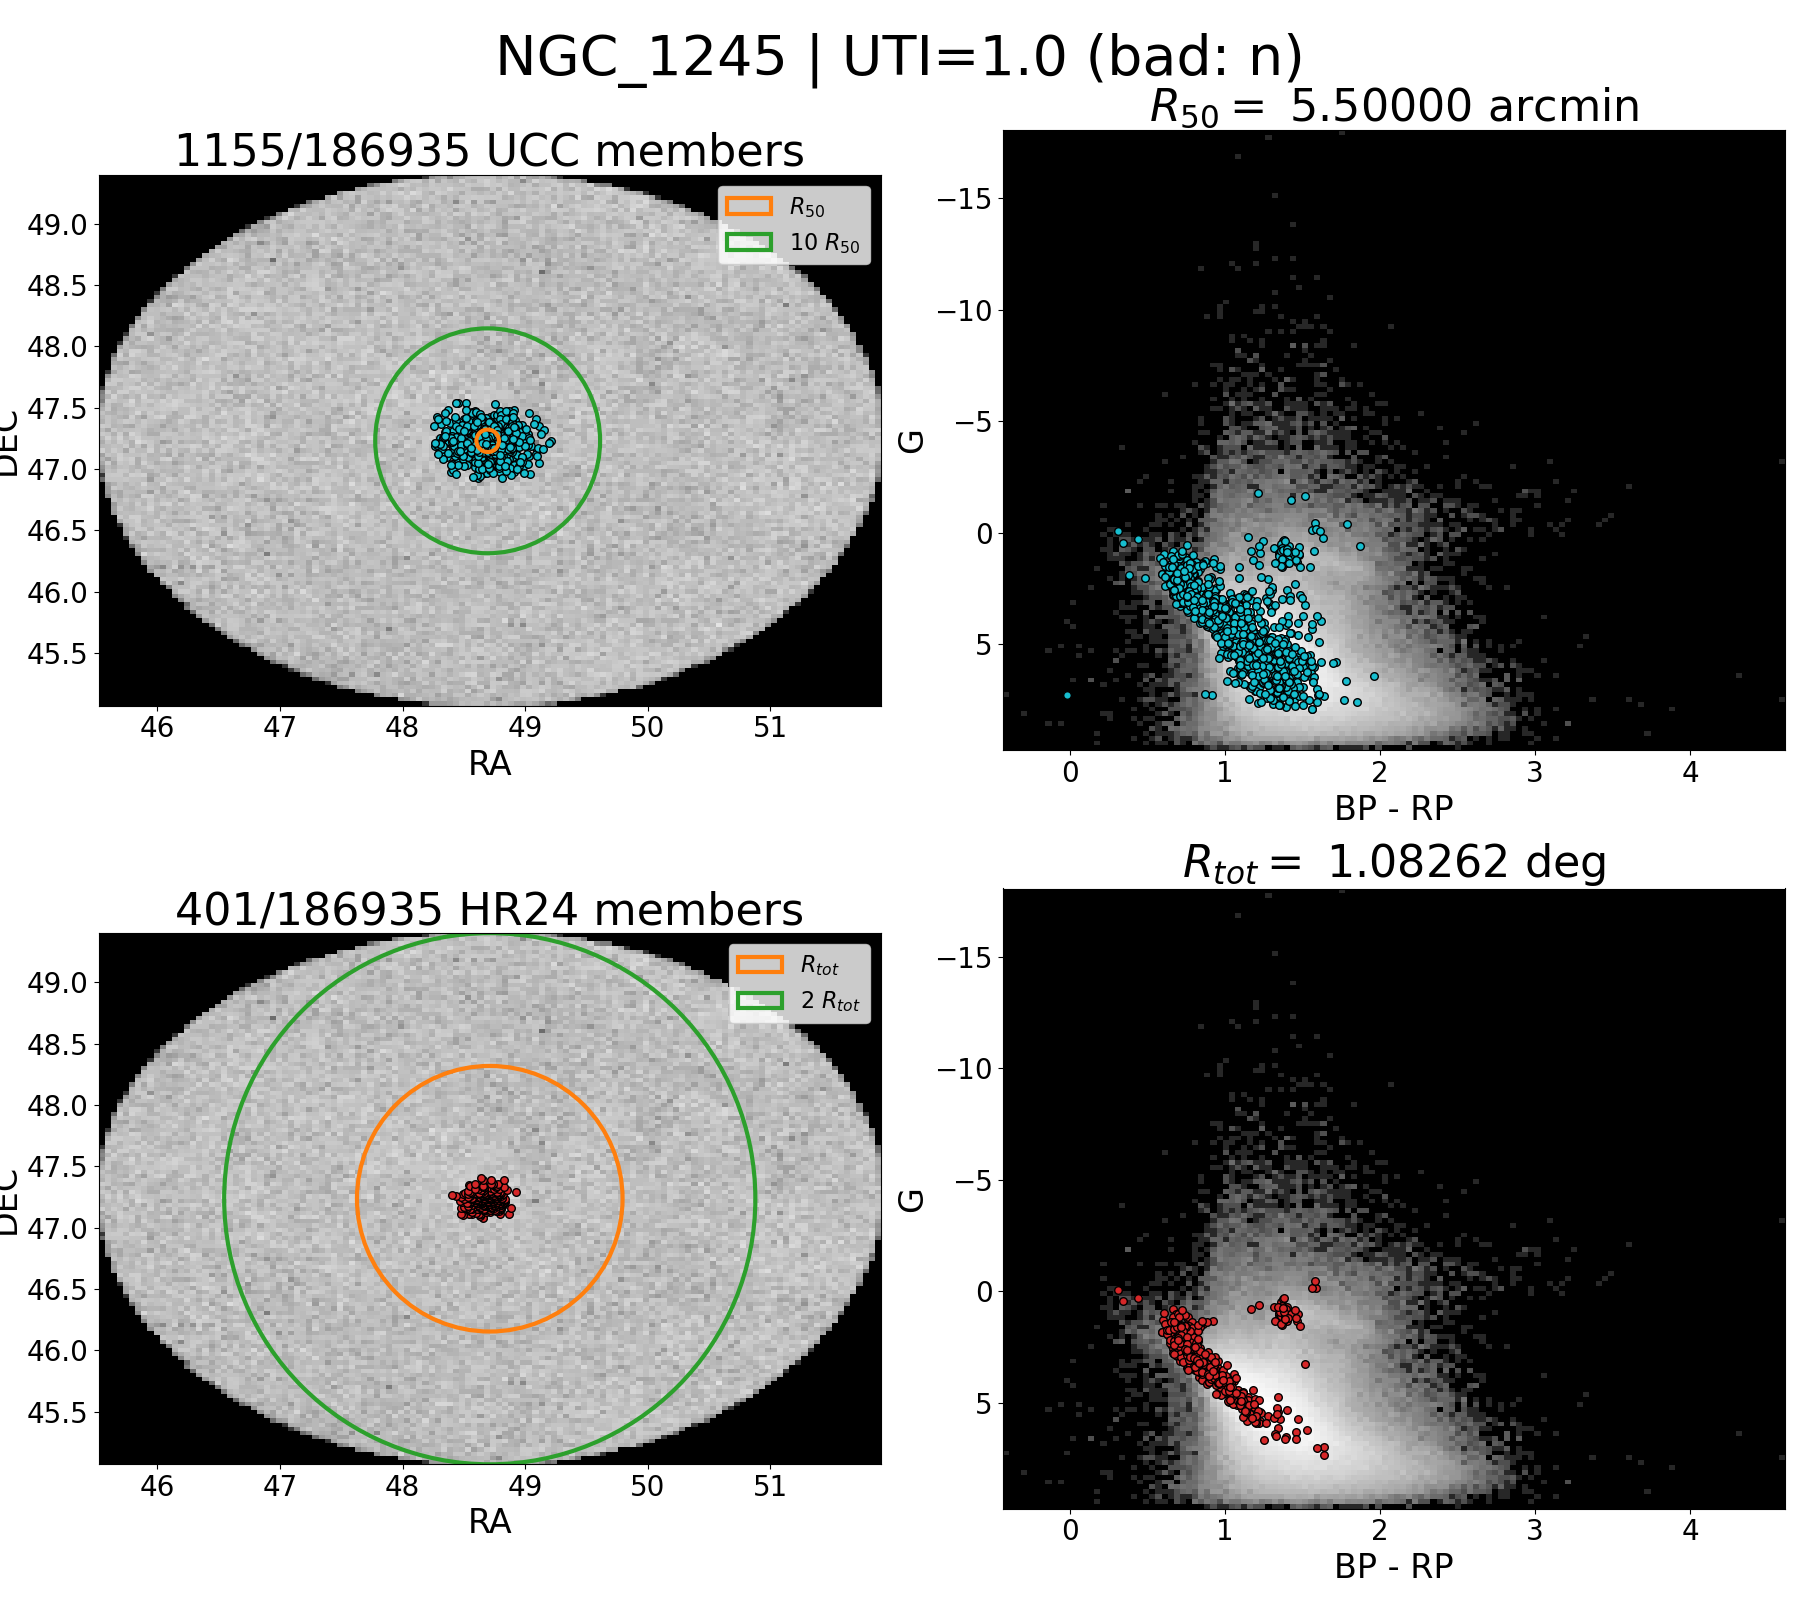
\includegraphics[width=0.495\linewidth]{figures/NGC_1245-radii.png}
    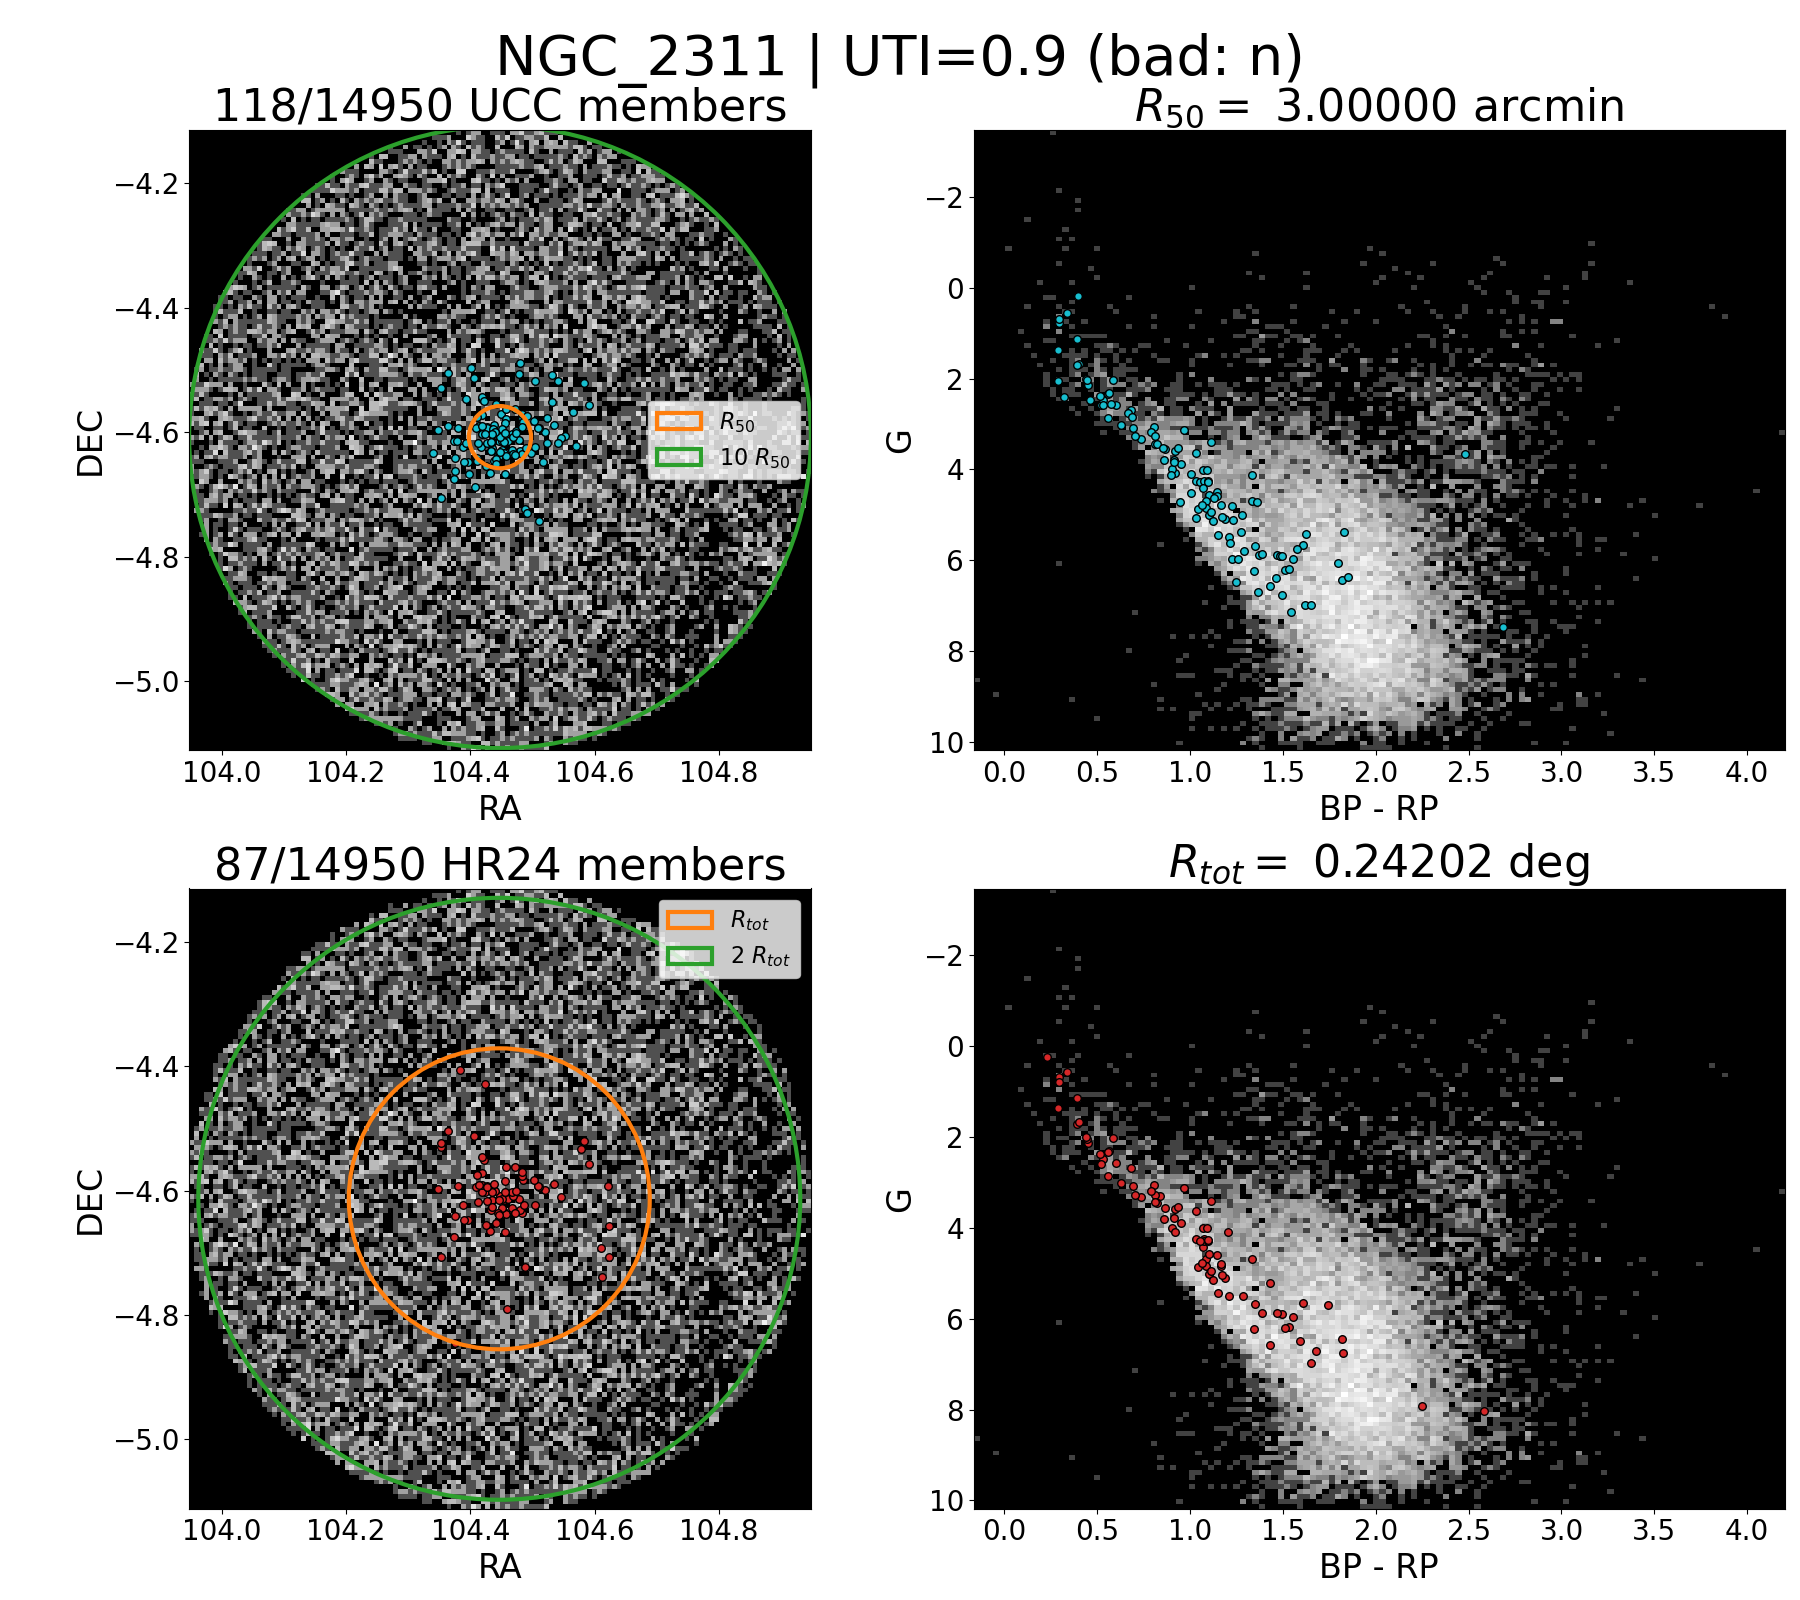
\includegraphics[width=0.495\linewidth]{figures/NGC_2311-radii.png}
    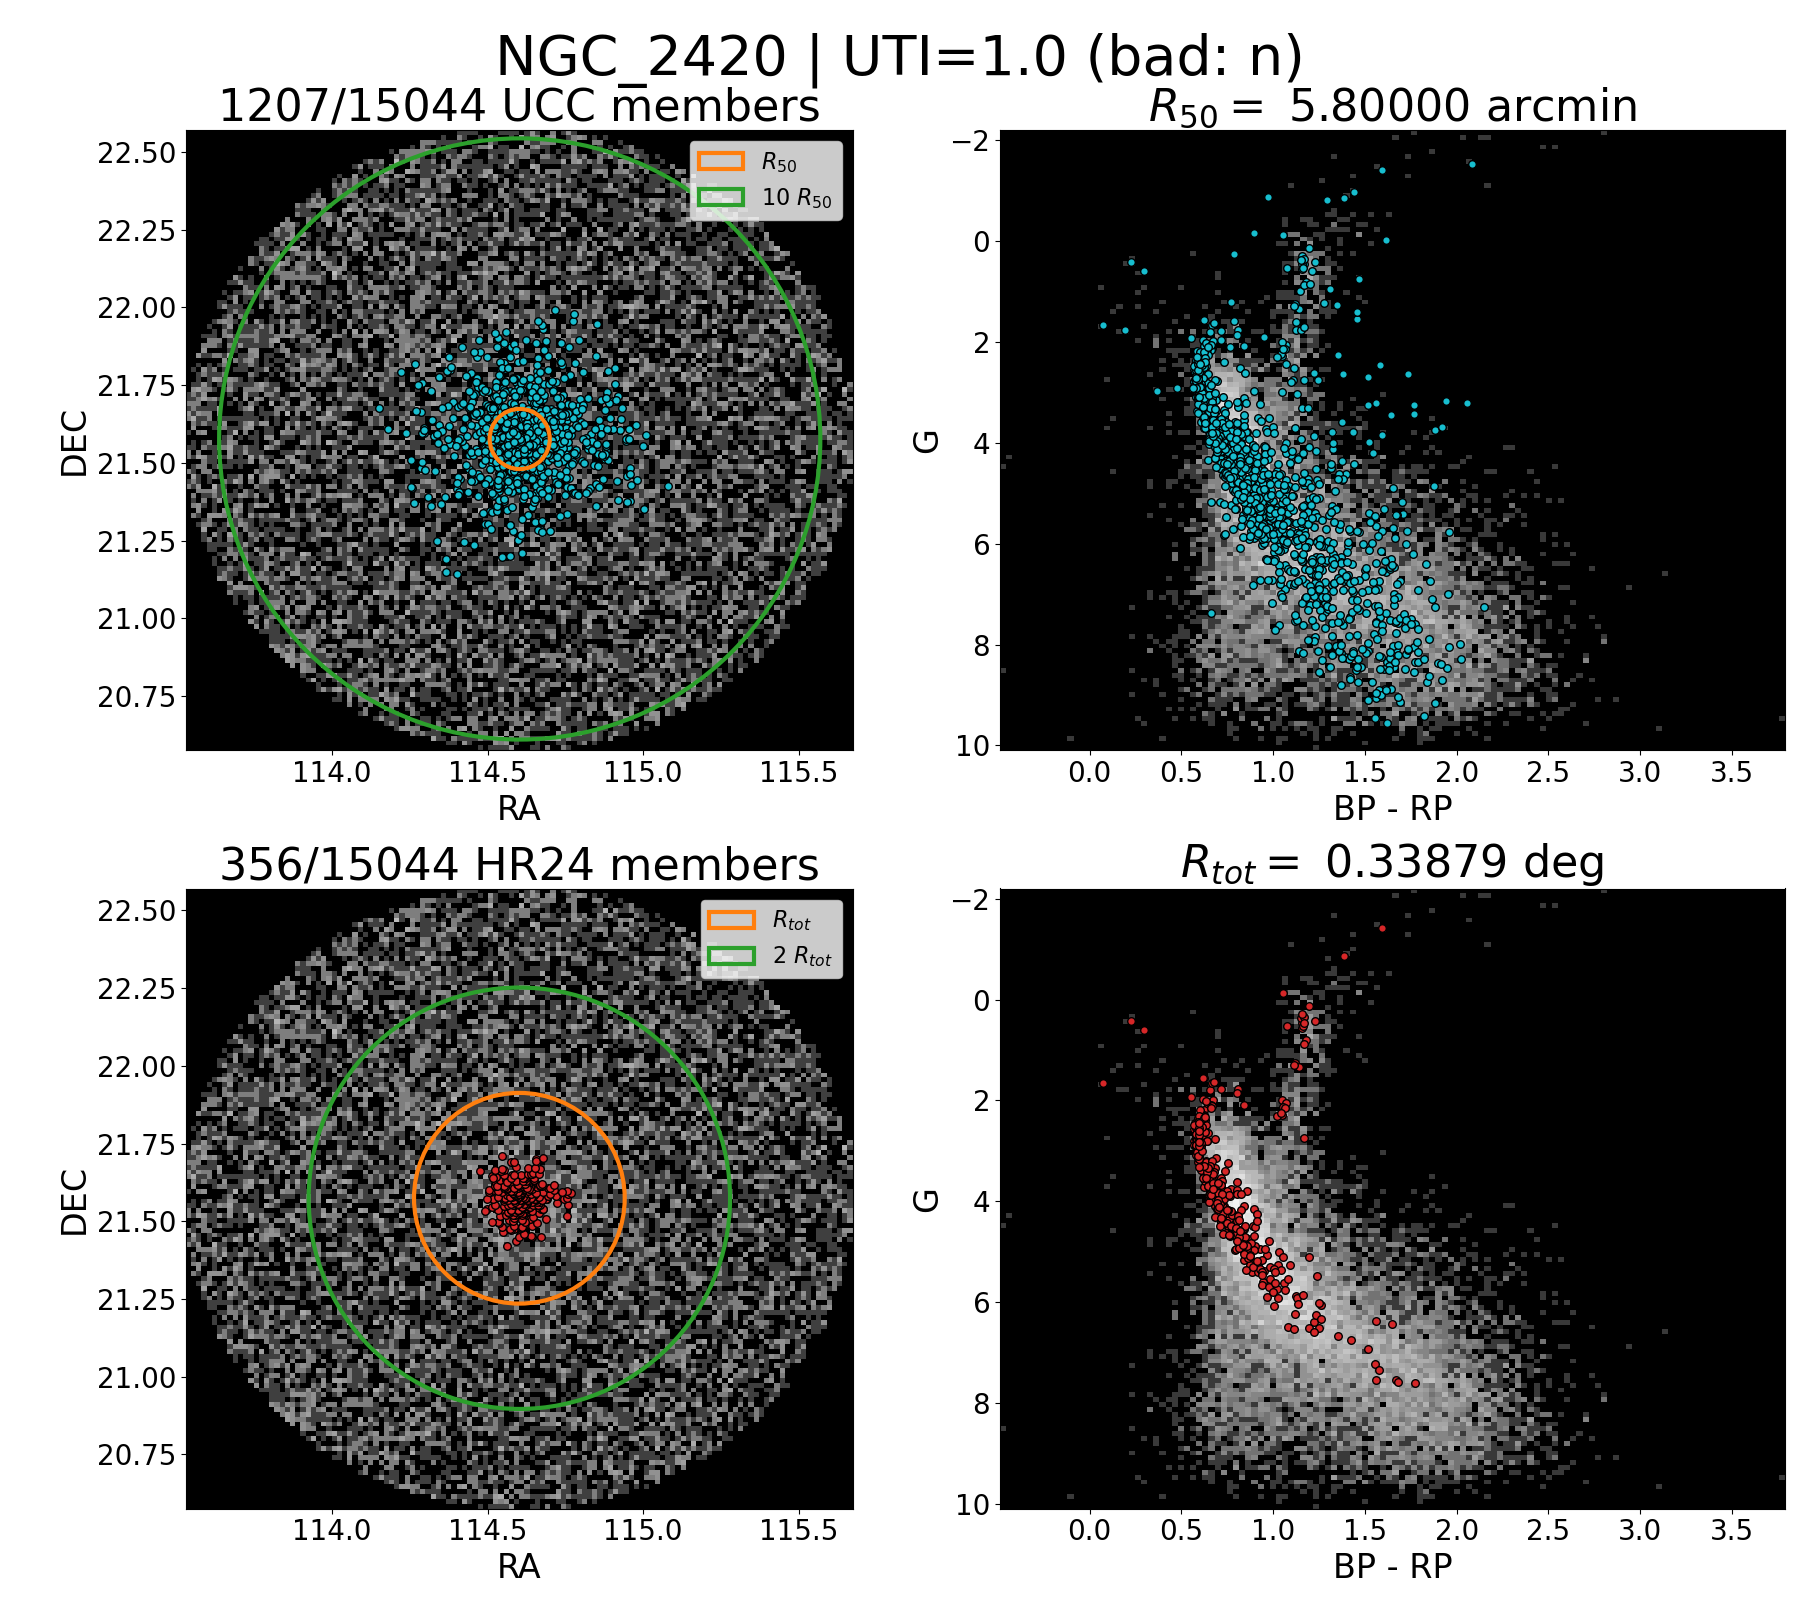
\includegraphics[width=0.495\linewidth]{figures/NGC_2420-radii.png}
    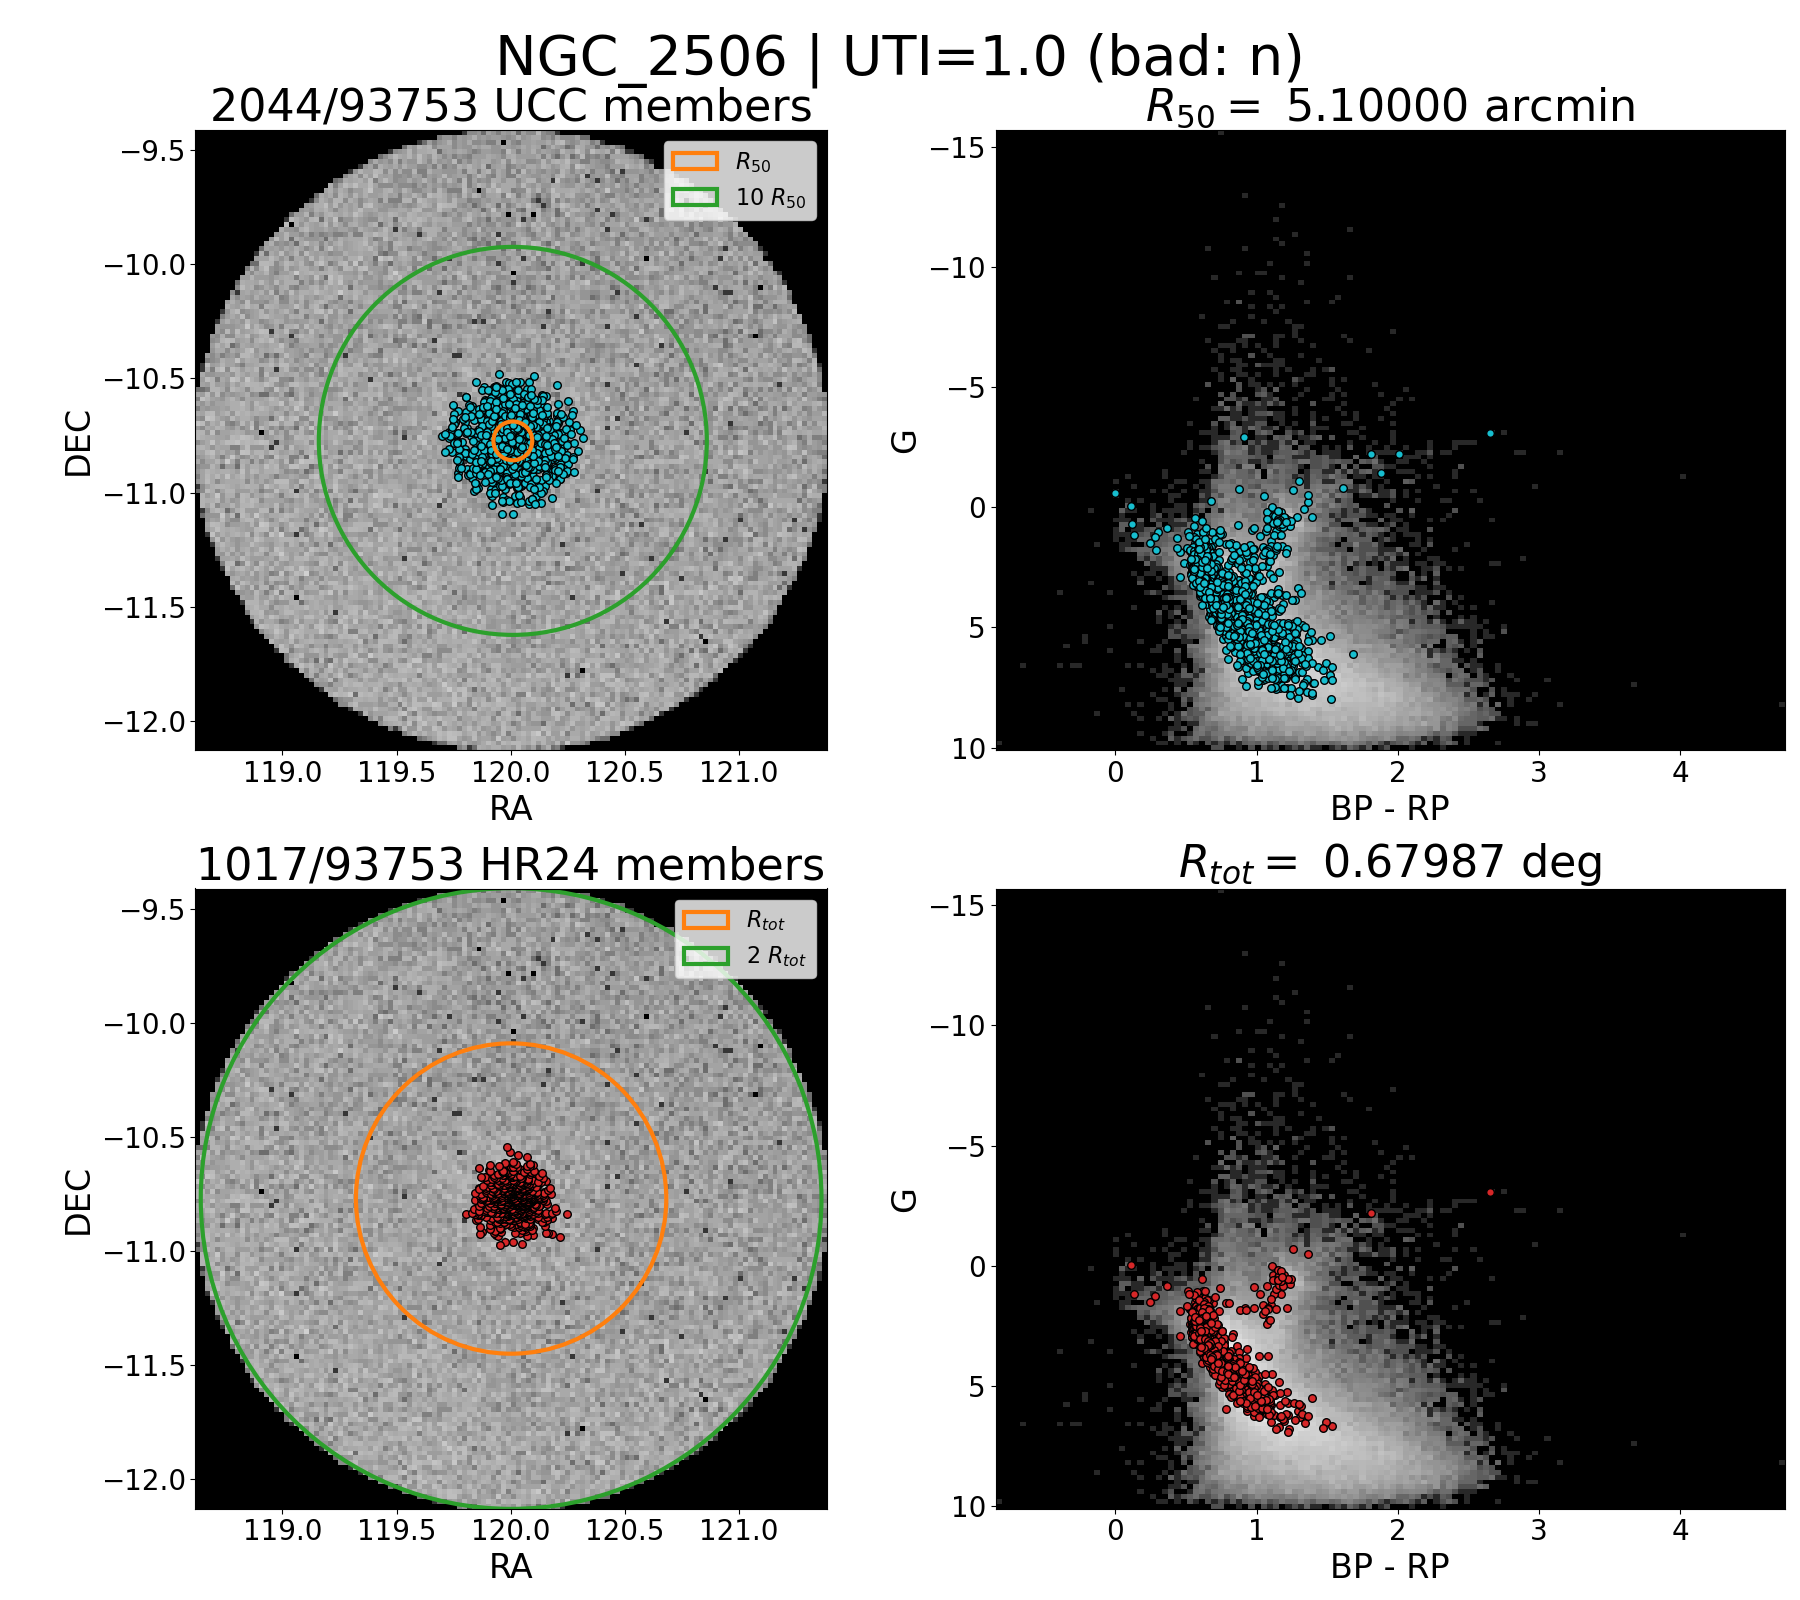
\includegraphics[width=0.495\linewidth]{figures/NGC_2506-radii.png}
    \caption{Gaia DR3 fields obtained using each OC's reported coordinates, with concentric rings denoting the search fields radii, along with the corresponding Gaia DR3 CMD. The upper panels of each OC overlays the reported cluster members in the UCC in blue, while the lower panels show the HR24 members overlaid in red.}
    \label{fig:gdr3-cone-search-fields}
\end{figure}

Each astrometric parameter was normalized to avoid the different scales of each parameter to overpower the other four dimensions, in particular to avoid issues with each field's parallax range, as its scale is order of magnitudes smaller than the other parameters. We performed a quality cut on our initial field sample by retrieving all stars in the field that satisfy $\code{fidelity\_v2} \geq 0.5$, where the \code{fidelity\_v2} flag is taken from \cite{rybizkiClassifierSpuriousAstrometric2022} characterizing whether each Gaia EDR3 astrometric solution is reliable. It has been previously used with success to discriminate cluster and star formation groups from a population of field stars without performing a hard cut on either magnitude or RUWE \autocite{huntImprovingOpenCluster2023a,rottensteinerComprehensiveClusterCensus2026}. 

\subsubsection{HDBSCAN Clustering}

Field star discrimination is performed using HDBSCAN \autocite{campelloDensityBasedClusteringBased2013}, a hierarchical density-based machine learning algorithm adept at finding clusters of data, whose hierarchical approach improves upon its predecessor DBSCAN's performance by not being biased towards a prescribed density. 

HDBSCAN takes two input parameters: a minimum number of neighboring points for a given cluster center ($m_{pts}$) and a minimum cluster size ($m_{cls}$) for a given data cluster is considered significant and not labeled as noise in the data. The membership determination pipeline in its current state runs the HDBSCAN clustering algorithm for a grid of $10 \leq m_{cls} \leq 5000$ in steps of 20. $m_{pts}$ was fixed to a value of 2 to reduce compute time, while the choice of $m_{pts} = 2$ was motivated to allow HDBSCAN to remain sensitive to more sparse clusters; when applied to more populated clusters such as NGC 1245, NGC 2311, NGC 2420, and NGC 2506, the hierarchical nature of HDBSCAN eventually collapses smaller groupings to a single cluster. 
% TODO: mention Average Centroid Linking Distance 